\subsection{Monocromatizar}

\subsubsection{Descripción}

\begin{wrapfigure}{r}{0.3\textwidth}
	\centering
	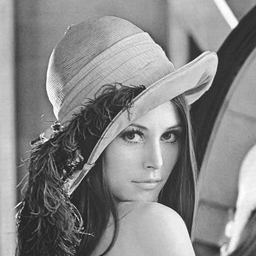
\includegraphics[width=0.3\textwidth]{imagenes/lenaMONO.jpg}
\end{wrapfigure}

El objetivo de este filtro es convertir una imagen color a una escala de grises. A diferencia de otros filtros, los pixeles de la imagen de salida estarán compuestos por un solo byte, que representará la intensidad de la luz. El criterio para obtener este valor es tomar el máximo entre los componentes R, G, B originales de cada pixel y aplicarlo al correspondiente en la imagen destino. Para esto aplicamos, a todos los pixeles de la imagen original, la siguiente función:

\begin{center}
	$I_{out}(p) = max(R, G, B)$
\end{center}

\hfill

\subsubsection{Implementación C}

A continuación el pseudocódigo de la implementación en C:

\begin{algorithm}[H]
  \begin{algorithmic}[1]
		\FORALL{y:=0 \TO  Height($I_{src}$)}
		 %\FOR x:=0 \TO  Width($I_{src}$)\STEP 1 \DO
			\FORALL{x:=0 \TO  Width($I_{src}$)}
			  \STATE $pixel \gets I_{src}(x,y)$
			  \STATE $Int$ $ r \gets Red(pixel) $
			  \STATE $Int$ $g \gets Green(pixel)$
			  \STATE $Int$ $ b \gets Blue(pixel)$
			  \STATE $Int$ $max \gets max(r, max(g, b))$
			  \STATE $pixel \gets DevolverPixel(r,g,b)$
			  \STATE $I_{dst}(x,y) \gets pixel$
			\ENDFOR
		 \ENDFOR
  \end{algorithmic}
  \caption{$monocromatizar (I_{src}, I_{dst})$}
  \label{alg:monocromatizar}
\end{algorithm}

\subsubsection{Implementación ASM}

En este filtro procesamos de a 4 píxeles en cada iteración usando las instrucciones \textbf{SSE} de la arquitectura. Por cada iteración se realizaron los cálculos del máximo de cada píxel y este se guardó en la imagen de salida.

\begin{itemize}

	\item En los registros \textbf{xmm0,xmm4, xmm5} tenemos la copia de los cuatro píxeles que levantamos de memoria. Y en \textbf{xmm1, xmm2, xmm3} las máscaras que usamos para los shuffles que luego utilizaremos para permutar los componentes.

		\begin{center}
		   \begin{tabular}{| c | c | c | c || c | c | c | c || c | c | c | c || c | c | c | c |}
			 \hline
			 a & b & g & r & a & b & g & r & a & b & g & r & a & b & g & r \\ \hline

		   \end{tabular}
		   \\ \textbf{xmm0, xmm4, xmm5}
		\end{center}
		 
		\begin{center}
		   \begin{tabular}{| c | c | c | c || c | c | c | c || c | c | c | c || c | c | c | c |}
			 \hline
			 15 & 13 & 13 & 13 & 11 & 9 & 9 & 9 & 7 & 5 & 5 & 5 & 3 & 1 & 1 & 1 \\ \hline
		   \end{tabular}
		   \\  \textbf{Mascara en xmm1 (mask1)}
		\end{center}

		\begin{center}
		   \begin{tabular}{| c | c | c | c || c | c | c | c || c | c | c | c || c | c | c | c |}
			 \hline
			 15 & 14 & 14 & 14 & 11 & 10 & 10 & 10 & 7 & 6 & 6 & 6 & 3 & 2 & 2 & 2 \\ \hline
		   \end{tabular}
		   \\ \textbf{Mascara en xmm2 (mask2)}
		\end{center}

		\begin{center}
		   \begin{tabular}{| c | c | c | c || c | c | c | c || c | c | c | c || c | c | c | c |}
			 \hline
			 15 & 12 & 12 & 12 & 11 & 8 & 8 & 8 & 7 & 4 & 4 & 4 & 3 & 0 & 0 & 0 \\ \hline
		   \end{tabular}
		   \\ \textbf{Mascara en xmm3(mask3)}
		\end{center}

	\item Realizamos el \textbf{shuffle xmm4, xmm1} que nos coloca el componente \textbf{g} en las posiciones que podemos observar en el registro xmm4. Y luego calculamos el máximo con la instrucción \textbf{pmaxub}. 

		\begin{center}
		   \begin{tabular}{| c | c | c | c || c | c | c | c || c | c | c | c || c | c | c | c |}
			 \hline
			 a & g & g & g & a & g & g & g & a & g & g & g & a & g & g & g \\ \hline
		   \end{tabular}
		   \\ \textbf{xmm4 $\gets$ pshufb xmm4, xmm1}
		\end{center}


		\begin{center}
		   \begin{tabular}{| c | c | c | c || c | c | c | c || c | c | c | c || c | c | c | c |}
			 \hline
			 a & . & . & max(g,r) & a & . & . & max(g,r) & a & . & . & max(g,r) & a & . & . & max(g,r)  \\ \hline
		   \end{tabular}
		   \\ \textbf{xmm4 $ \gets $ pmaxub xmm4, xmm0}
		\end{center}

	\item Realizamos el mismo procedimiento en este paso. Luego nos quedaría el valor del máximo (ver imagen). 
		\begin{center}
		   \begin{tabular}{| c | c | c | c || c | c | c | c || c | c | c | c || c | c | c | c |}
			 \hline
			 a & b & b & b & a & b & b & b & a & b & b & b & a & b & b & b \\ \hline
		   \end{tabular}
		   \\ \textbf{xmm5 $\gets$ pshufb xmm5, xmm2}
		\end{center}

		\begin{center}
		   \begin{tabular}{| c | c | c | c || c | c | c | c || c | c | c | c || c | c | c | c |}
			 \hline
			 a & . & . & max(g,r,b) & a & . & . & max(g,r,b) & a & . & . & max(g,r,b) & a & . & . & max(g,r,b)  \\ \hline
		   \end{tabular}
		   \\ \textbf{xmm4 $\gets$ pmaxub xmm4, xmm5}
		\end{center}


	\item Solo resta copiar los máximos. Para esto utilizaremos el shuffle junto con la máscara contenida en xmm3.

		\begin{center}
		   \begin{tabular}{| c | c | c | c || c | c | c | c || c | c | c | c || c | c | c | c |}
			 \hline
			 a & max & max & max & a & max & max & max & a & max & max & max & a & max & max & max  \\ \hline
		   \end{tabular}
		   \\ \textbf{xmm5 $\gets$ pshufb xmm4, xmm3}
		\end{center}

\end{itemize}

Por último resta copiar esto a memoria, brindamos el código ASM de este paso.

\begin{codesnippet}
\begin{verbatim}
section .data
    mask1: db 1, 1, 1, 3, 5, 5, 5, 7, 9, 9, 9, 11, 13, 13, 13, 15
    mask2: db 2, 2, 2, 3, 6, 6, 6, 7, 10, 10, 10, 11, 14, 14, 14, 15
    mask3: db 0, 0, 0, 3, 4, 4, 4, 7, 8, 8, 8, 11, 12, 12, 12, 15

section .text

monocromatizar_inf_asm:
    ...
    movdqu xmm0, [rdi]  ; xmm0=|a b g r|a b g r|a b g r|a b g r|
    movdqu xmm4, xmm0   ; xmm4= xmm0
    movdqu xmm5, xmm0   ; xmm5= xmm0

    pshufb xmm4, xmm1   ; xmm4=|a g g g|a g g g|a g g g|a g g g|
    pmaxub xmm4, xmm0   ; xmm4=|a . . max(g,r)|a . . max(g,r)|a . . max(g,r)|a . . max(g,r)|;1er máximo

    pshufb xmm5, xmm2   ; xmm5=|a b b b|a b b b|a b b b|a b b b|			
    pmaxub xmm4, xmm5   ; xmm4=|a . . max(g,r,b)|a . . max(g,r,b)|a . . max(g,r,b)|;máx de máximos
                        ; xmm4=|a . . max|a . . max|a . . max|a . . max|	
    pshufb xmm4, xmm3   ; xmm4=|a max max max|a max max max|a max max max|a max max max|

    movdqu [rsi], xmm4  ; [rsi]= xmm4
    ...
\end{verbatim}
\end{codesnippet}
